\section{梯度估计的方差控制}
\label{sec:pgrad-variance}

前三节得到了同一个梯度的几种表示。以$X\sim\mathcal{N}(\theta,1)$、$f(x)=x^{2}$为例，路径导数$2X$与得分估计$X^{2}(X-\theta)$的期望都是$2\theta$，它们是同一个向量期望的不同计算公式。第~\ref{chap:variance-reduction}章的观点在这里完全适用：期望相同的计算公式之间可以比较方差，也可以用控制变量和条件期望改造公式，只要改造不改变期望。

\paragraph{比较的对象}

梯度估计是$\mathbb{R}^{k}$值的，单样本$\bm{G}$的波动由协方差矩阵$\bm{\Sigma}_{\bm{G}}$描述。比较两个估计时，可以逐分量比较方差$(\bm{\Sigma}_{\bm{G}})_{j,j}$，也可以沿指定方向$\bm{u}$比较
\[
  \operatorname{Var}\bigl(\langle\bm{u},\bm{G}\rangle\bigr)=\bm{u}^{\top}\bm{\Sigma}_{\bm{G}}\bm{u},
\]
或比较式~\eqref{eq:pgrad-direct-mse}中的迹。不同分量的精度可以相差很大，第~\ref{sec:pgrad-reparam}节的高斯例子里，$\mu$分量与$\sigma$分量的单样本方差分别是$1$和$6$。这些比较都以$\mathbb{E}\lVert\bm{G}\rVert_{2}^{2}<\infty$为前提，要对每个用到的分量分别核对。

先把高斯例子的两个方差算出来。重参数化的单样本$2X$方差为$4$。得分估计是$X^{2}\varepsilon$，其中$\varepsilon=X-\theta$。求它的二阶矩要展开$(\theta+\varepsilon)^{4}\varepsilon^{2}$，所用的标准正态矩是
\[
  \mathbb{E}[\varepsilon^{2}]=1,\qquad\mathbb{E}[\varepsilon^{4}]=3,\qquad\mathbb{E}[\varepsilon^{6}]=15,
\]
奇数阶矩为零。只保留偶数次项，得到
\[
  \mathbb{E}\bigl[(\theta+\varepsilon)^{4}\varepsilon^{2}\bigr]=\theta^{4}+6\theta^{2}\cdot3+15=\theta^{4}+18\theta^{2}+15 .
\]
减去均值的平方$4\theta^{2}$，方差为$\theta^{4}+14\theta^{2}+15$。在$\theta=1$处是$30$，约为重参数化的$7.5$倍：要达到同样的精度，得分估计需要约$7.5$倍的样本。

\paragraph{得分作为控制变量}

得分估计的方差大，一个原因可以直接看出。由第~\ref{chap:information-geometry}章，正则族的得分期望为零。于是对任意常数$b$，
\[
  \mathbb{E}\bigl[(f(X)-b)\,s(X)\bigr]=\mathbb{E}[f(X)s(X)]-b\,\mathbb{E}[s(X)]=\mathbb{E}[f(X)s(X)],
\]
期望不变。项$b\,s(X)$是纯粹的噪声：它的平均为零，却随样本上下波动。在高斯例子里$f=X^{2}$总是正的，$f s$的波动有相当一部分来自$f$的平均水平乘上$s$的符号；减去一个接近$f$平均水平的$b$，就把这部分去掉了。这个常数$b$称为\term{基线}（baseline）。

这正是第~\ref{chap:variance-reduction}章的控制变量：辅助函数$h=s_{j}$的期望已知为零，系数为$b$。各分量可以用不同的基线$b_{j}$。若$\mathbb{E}[f^{2}s_{j}^{2}]<\infty$且$0<\mathbb{E}[s_{j}^{2}]<\infty$，第$j$个分量的方差是
\[
  V_{j}(b_{j})=\mathbb{E}\bigl[(f-b_{j})^{2}s_{j}^{2}\bigr]-\bigl(\mathbb{E}[f s_{j}]\bigr)^{2},
\]
它是$b_{j}$的二次函数。对$b_{j}$求导并令其为零，$-2\mathbb{E}[(f-b_{j})s_{j}^{2}]=0$，得到最优基线
\begin{equation}
  b_{j}^{*}=\frac{\mathbb{E}\bigl[f(X)\,s_{j}(X)^{2}\bigr]}{\mathbb{E}\bigl[s_{j}(X)^{2}\bigr]}.
  \label{eq:pgrad-optimal-baseline}
\end{equation}
它是按$s_{j}^{2}$加权的$f$的平均：得分大的样本对估计影响大，基线应当贴近这些样本上的函数值。由于$\mathbb{E}[s_{j}]=0$，它与控制变量的最优系数$\operatorname{Cov}(fs_{j},s_{j})/\operatorname{Var}(s_{j})$一致。

在高斯例子中，同样只保留偶数次项，
\[
  \mathbb{E}[f s^{2}]=\mathbb{E}\bigl[(\theta+\varepsilon)^{2}\varepsilon^{2}\bigr]=\theta^{2}+3,\qquad\mathbb{E}[s^{2}]=1,
\]
所以$b^{*}=\theta^{2}+3$。在$\theta=1$处，前面算出的$\mathbb{E}[f^{2}s^{2}]$等于$34$，方差作为$b$的函数是
\[
  V(b)=34-8b+b^{2}-4=b^{2}-8b+30 .
\]
三个基线的结果是
\[
  V(0)=30,\qquad V(J(1))=V(2)=18,\qquad V(b^{*})=V(4)=14 .
\]
用$J(\theta)=\mathbb{E}[f]$作基线是常见的简便选择，这里它把方差从$30$降到$18$；最优基线降到$14$。图~\ref{fig:pgrad-baseline-var}画出了这条抛物线。即使用最优基线，得分估计仍不如重参数化的$4$：常数基线只能去掉与$s$成比例的那部分噪声。

\begin{BookInlineFigure}
  \centering
  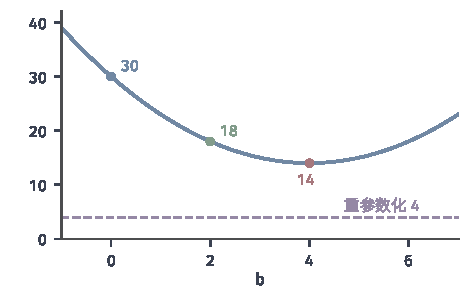
\includegraphics[width=80mm]{figures/07-probability/08-sampling-and-integration/matplotlib/pgrad-baseline-var/figure.pdf}
  \caption{$X\sim\mathcal{N}(1,1)$，$f(x)=x^{2}$。单样本估计$(f(X)-b)(X-1)$的方差$V(b)=b^{2}-8b+30$（蓝线）。蓝点为无基线$b=0$，绿点为$b=J(1)=2$，红点为最优基线$b^{*}=4$；紫色虚线为重参数化估计$2X$的方差$4$。}
  \label{fig:pgrad-baseline-var}
\end{BookInlineFigure}

\paragraph{基线所用的数据}

最优基线含有未知的期望，实际中要用样本估计。这时必须注意：$\mathbb{E}[b\,s(X)]=0$的推导要求$b$是常数，或者至少与$X$独立。若$b$由与当前样本独立的数据算出（例如先前单独抽取的一批试运行样本），则在给定这批数据的条件下$b$是常数，估计条件无偏，因而无偏。若$b$用到了当前样本本身，就要重新检查。

最自然的错误是用全部样本的平均$\bar{F}=\frac{1}{n}\sum_{j}f(X_{j})$作基线。对第$i$项，
\[
  \mathbb{E}\bigl[\bar{F}s(X_{i})\bigr]=\frac{1}{n}\mathbb{E}\bigl[f(X_{i})s(X_{i})\bigr]+\frac{1}{n}\sum_{j\neq i}\mathbb{E}[f(X_{j})]\,\mathbb{E}[s(X_{i})]=\frac{1}{n}J'(\theta),
\]
因为$\bar{F}$里含有$f(X_{i})$，它与$s(X_{i})$相关。于是
\[
  \mathbb{E}\bigl[(f(X_{i})-\bar{F})\,s(X_{i})\bigr]=\Bigl(1-\frac{1}{n}\Bigr)J'(\theta),
\]
估计系统地偏小。这和第~\ref{sec:pgrad-cov-sample}节样本协方差的偏差是同一个来源。

修正的办法是让每个样本的基线不含它自己：用其余$n-1$个样本的平均
\[
  b_{i}=\bar{F}_{-i}=\frac{1}{n-1}\sum_{j\neq i}f(X_{j}),
\]
称为\term{留一基线}（leave-one-out baseline）。$b_{i}$与$X_{i}$独立，所以$\mathbb{E}[(f(X_{i})-b_{i})s(X_{i})]=J'(\theta)$，估计无偏。由$\bar{F}_{-i}=(n\bar{F}-f(X_{i}))/(n-1)$，直接算出
\[
  f(X_{i})-\bar{F}_{-i}=\frac{n}{n-1}\bigl(f(X_{i})-\bar{F}\bigr),
\]
所以留一基线的估计恰好是全平均基线估计乘以$\frac{n}{n-1}$，与样本协方差的$n-1$分母是同一个修正。

下面用固定噪声手算。$\theta=1$，$\varepsilon=0.3,-1.1,0.8,-0.4$，样本$X=1.3,\,-0.1,\,1.8,\,0.6$，函数值与得分为
\[
  f=1.69,\ 0.01,\ 3.24,\ 0.36,\qquad s=0.3,\ -1.1,\ 0.8,\ -0.4 .
\]
不用基线时，$f s=0.507,\ -0.011,\ 2.592,\ -0.144$，平均为$0.736$。全平均为$\bar{F}=1.325$，四个留一基线是
\[
  b_{i}=1.2033,\ 1.7633,\ 0.6867,\ 1.6467,
\]
对应的$(f-b_{i})s=0.1460,\ 1.9287,\ 2.0427,\ 0.5147$，平均为$1.158$。用全平均作基线得到$0.8685$，正好是$1.158\times\frac{3}{4}$。真值是$2$。四个样本太少，三者都偏离真值，但只有前两种在平均意义下是无偏的。图~\ref{fig:pgrad-loo-baseline}用大量重复验证了全平均基线的偏差因子$\frac{n-1}{n}$。

\begin{BookInlineFigure}
  \centering
  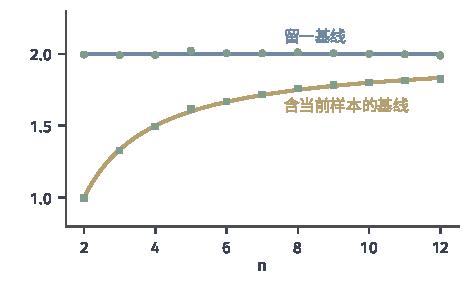
\includegraphics[width=80mm]{figures/07-probability/08-sampling-and-integration/matplotlib/pgrad-loo-baseline/figure.pdf}
  \caption{$X\sim\mathcal{N}(1,1)$，$f(x)=x^{2}$，真值$J'(1)=2$。蓝线与绿色圆点：留一基线估计的期望（恒为$2$）；黄线与绿色方块：以含当前样本的全平均作基线的估计，期望为$2(n-1)/n$。线为精确值，点为每个$n$重复$40000$次（固定种子）的平均。}
  \label{fig:pgrad-loo-baseline}
\end{BookInlineFigure}

教训是：依赖当前样本的修正不能默认无偏。留一基线之所以无偏，是因为每一项的基线与该项的得分独立；任意用当前样本拟合出来的修正项都要像上面这样逐项核对期望。

\paragraph{条件期望}

第~\ref{chap:variance-reduction}章的另一种方法是把能解析算出的随机性先积掉。设$X=(X_{1},X_{2})$，$X_{1}\sim\mathcal{N}(\theta,1)$与$X_{2}\sim\mathcal{N}(0,1)$独立，$f(x)=x_{1}^{2}+x_{2}^{2}$。参数只在$X_{1}$的分布里，得分是$s=X_{1}-\theta$，单样本得分估计为$(X_{1}^{2}+X_{2}^{2})(X_{1}-\theta)$。其中$X_{2}^{2}$与参数无关，却乘在$s$上增加波动。给定$X_{1}$对$X_{2}$取条件期望，$\mathbb{E}[X_{2}^{2}]=1$，得到改造后的估计
\[
  \mathbb{E}\bigl[(X_{1}^{2}+X_{2}^{2})s\mid X_{1}\bigr]=(X_{1}^{2}+1)(X_{1}-\theta).
\]

期望不变。记原估计为$G$，由全方差公式，方差减少的量是
\[
  \mathbb{E}\bigl[\operatorname{Var}(G\mid X_{1})\bigr]=\mathbb{E}[s^{2}]\operatorname{Var}(X_{2}^{2})=1\cdot2=2 .
\]
在$\theta=1$处可以直接核对。记$f_{1}=X_{1}^{2}$，前面已经算出$f_{1}^{2}s^{2}$与$f_{1}s^{2}$的期望分别是$34$与$4$；又$X_{2}^{2}$与$X_{2}^{4}$的期望分别是$1$与$3$。展开平方后逐项取期望，两个估计的二阶矩分别是
\[
  34+2\cdot4\cdot1+3\cdot1=45,\qquad34+2\cdot4+1=43,
\]
减去$J'(1)^{2}=4$后方差为$41$与$39$。条件化与基线可以叠加使用：在$(X_{1}^{2}+1)s$上再减去基线，就回到了一维问题的抛物线。

\paragraph{两种表示哪个更好}

在高斯二次函数的例子里，重参数化全面占优。从图~\ref{fig:pgrad-variance-compare}(a)可以看到，在$\theta\in[-2,2]$上它的方差恒为$4$，而得分估计即使配上最优基线也在$6$以上，并随$\lvert\theta\rvert$增长。但这不是普遍规律。路径导数用到$f$对$x$的导数，$f$变化剧烈时这个导数会放大波动；得分估计只用到$f$的值。

取$f(x)=\sin(\omega x)$，$X\sim\mathcal{N}(\theta,1)$。路径导数是$\omega\cos(\omega X)$，幅度随$\omega$增大；得分估计是$\sin(\omega X)(X-\theta)$，$\lvert\sin\rvert\leq1$限制了它。计算方差要用到两个高斯积分：
\[
  \mathbb{E}[\cos(cX)]=\mathrm{e}^{-c^{2}/2}\cos(c\theta),\qquad\mathbb{E}\bigl[\varepsilon^{2}\mathrm{e}^{\mathrm{i}c\varepsilon}\bigr]=(1-c^{2})\mathrm{e}^{-c^{2}/2},
\]
后者是标准正态特征函数$\mathrm{e}^{-c^{2}/2}$的二阶导数取负号。再用倍角公式把$\cos^{2}(\omega X)$与$\sin^{2}(\omega X)$写成$\cos(2\omega X)$的线性函数，在$\theta=0$处两者的方差为
\begin{align}
  \operatorname{Var}_{\mathrm{rep}}&=\frac{\omega^{2}}{2}\bigl(1+\mathrm{e}^{-2\omega^{2}}\bigr)-\omega^{2}\mathrm{e}^{-\omega^{2}},\label{eq:pgrad-sin-rep}\\
  \operatorname{Var}_{\mathrm{sf}}&=\frac{1}{2}\bigl(1-(1-4\omega^{2})\mathrm{e}^{-2\omega^{2}}\bigr)-\omega^{2}\mathrm{e}^{-\omega^{2}}.\label{eq:pgrad-sin-sf}
\end{align}

两式中减去的$\omega^{2}\mathrm{e}^{-\omega^{2}}$是$J'(0)^{2}$。$\omega\to\infty$时式~\eqref{eq:pgrad-sin-rep}像$\omega^{2}/2$那样增长，式~\eqref{eq:pgrad-sin-sf}趋于$\frac{1}{2}$。图~\ref{fig:pgrad-variance-compare}(b)显示两条曲线在$\omega\approx1.12$处相交，此后得分估计更好。

\begin{BookInlineFigure}
  \centering
  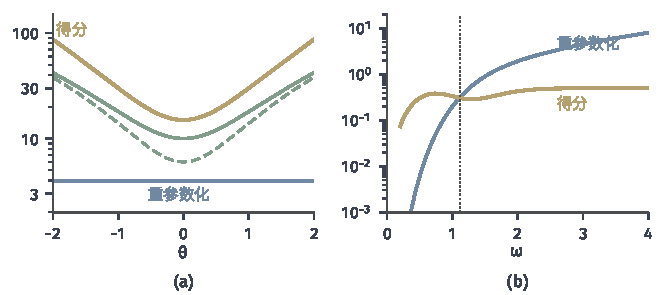
\includegraphics[width=112mm]{figures/07-probability/08-sampling-and-integration/matplotlib/pgrad-variance-compare/figure.pdf}
  \caption{$X\sim\mathcal{N}(\theta,1)$时单样本梯度估计的方差（对数纵轴）。(a)$f(x)=x^{2}$：蓝线为重参数化（恒为$4$），黄线为得分估计$\theta^{4}+14\theta^{2}+15$，绿实线为以$J(\theta)$为基线的得分估计$8\theta^{2}+10$，绿虚线为最优基线下的$8\theta^{2}+6$。(b)$f(x)=\sin(\omega x)$，$\theta=0$：蓝线为式~\eqref{eq:pgrad-sin-rep}，黄线为式~\eqref{eq:pgrad-sin-sf}，点线标出交点$\omega\approx1.12$。}
  \label{fig:pgrad-variance-compare}
\end{BookInlineFigure}

所以选择表示时不能预设哪一种更好。可用性由前几节的条件决定：函数沿路径是否受Lipschitz控制，得分能否计算，支撑是否随参数移动。在都可用的情形下，比较的是同一梯度任务下的方差与单样本成本；把这一比较放进整体预算，是下一章的内容。
